\documentclass{standalone}
\usepackage{fontspec}
\usepackage{tikz}
\usetikzlibrary{decorations,decorations.pathreplacing}
\usepackage{bm}
\renewcommand*\familydefault{\sfdefault}
%\usepackage{sansmath}%\usepackage{arev}
\usepackage[italic]{mathastext}
\usepackage{isomath}
%\setromanfont{CMU Sans Serif}

\begin{document}
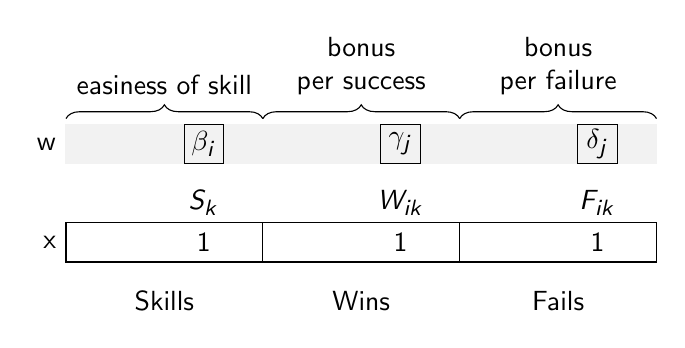
\begin{tikzpicture}[scale=0.5]
\filldraw[gray!10!white] (0,2.5) rectangle ++(15,1);
\draw (0,0) rectangle (15,1);
\draw node[left] at (0,0.5) {$\bm{x}$};
\draw node[left] at (0,3) {$\bm{w}$};

\node at (3.5,0.5) {1};
\node at (3.5,3) {$\beta_i$};
\draw[decorate,decoration={brace,raise=2pt,amplitude=5pt}] (0,3.5) -- (5,3.5);
\node[above] at (2.5,4) {easiness of skill};
\draw[decorate,decoration={brace,raise=2pt,amplitude=5pt}] (5,3.5) -- (10,3.5);
\node[above,text centered,text width=2cm] at (7.5,4) {bonus\\per success};
\draw[decorate,decoration={brace,raise=2pt,amplitude=5pt}] (10,3.5) -- (15,3.5);
\node[above,text centered,text width=2cm] at (12.5,4) {bonus\\per failure};

\node at (8.5,0.5) {1};
\node at (13.5,0.5) {1};
\node at (8.5,3) {$\gamma_j$};
\draw (8,2.5) rectangle ++(1,1);
\node at (13.5,3) {$\delta_j$};
\draw (13,2.5) rectangle ++(1,1);
\node at (3.5,1.5) {$S_k$};
\node at (8.5,1.5) {$W_{ik}$};
\node at (13.5,1.5) {$F_{ik}$};

% Highlight
\draw (3,2.5) rectangle ++(1,1);
\draw (5,0) -- ++(0,1);
\draw (10,0) -- ++(0,1);
\node at (2.5,-1) {Skills};
% \node at (5,4) {$\theta$};
\node at (7.5,-1) {Wins};
\node at (12.5,-1) {Fails};
% \node at (13,4) {$e$};
%\draw (3,4) rectangle ++(1,3);
\end{tikzpicture}
\end{document}
